 \documentclass[c]{beamer}
%\documentclass{beamer}
\listfiles

\mode<presentation>
{
  %\usetheme[deutsch,titlepage0]{KIT}
\usetheme[deutsch]{KIT}
% \usetheme{KIT}

%%  \usefonttheme{structurebold}

  \setbeamercovered{transparent}

  \setbeamertemplate{enumerate items}[circle]
  %\setbeamertemplate{enumerate items}[ball]

}
\usepackage{babel}
\date{}
%\DateText

\newlength{\Ku}
\setlength{\Ku}{1.43375pt}

\usepackage[utf8]{inputenc}
\usepackage[TS1,T1]{fontenc}
\usepackage{array}
\usepackage{multicol}
\usepackage{lipsum}
\usepackage[]{algorithm2e}
\usepackage{amsmath}
\usepackage{color}

\usenavigationsymbols
%\usenavigationsymbols[sfHhdb]
%\usenavigationsymbols[sfhHb]

\subtitle{Algorithmen I SS 14}
\author[]{Vincent Schüßler}

\AuthorTitleSep{\relax}

\institute[ITI]{Institut für Theoretische Informatik}

\TitleImage[width=\titleimagewd]{images/title}

\newlength{\tmplen}

\newcommand{\verysmall}{\fontsize{6pt}{8.6pt}\selectfont}

\title[Algorithmen I SS 14]{Tutorium 10}

\usepackage{alltt}

\TitleImage[width=\titleimagewd]{images/title02}

\begin{document}

\begin{frame}
  \maketitle
\end{frame}

\begin{frame}
	\begin{center}
		\Huge
		Kürzeste Wege
	\end{center}
\end{frame}

\begin{frame}{Bellman-Ford: Einsatz}
	\begin{itemize}
		\item Wie Dijkstra: Finden der kürzesten Wege vom Startknoten zu allen anderen Knoten (single-source shortest paths)
		\item auch mit negativen Kantengewichten
		\item insbesondere Finden von negativen Kreisen im Graphen
	\end{itemize}
\end{frame}

\begin{frame}{Bellman-Ford-Algorithmus: Idee}
	\begin{itemize}
		\item kürzeste Wege können maximal die Länge $|V|-1$ haben
		\item die kürzesten Wege mit Länge k+1 sind aus denen der Länge k berechenbar
	\end{itemize}
\end{frame}

\begin{frame}{Bellman-Ford: Algorithmus}
	\begin{enumerate}
		\item Initialisiere die Knotendistanz $d$ des Startknotens mit 0 alle anderen mit $\infty$.
		\item Iteriere $|V|-1$-mal über alle Kanten:
			\begin{itemize}
				\item Ist $d_v > d_u + $ Kantengewicht $e_{(u,v)}$, dann aktualisiere $d_v$
			\end{itemize}
		\item Iteriere nocheinmal über die Kanten. Ändern sich Werte so gibt es einen negativen Kreis
	\end{enumerate}
	$\Rightarrow$ Laufzeit $ O(|V||E|)$
\end{frame}


\begin{frame}{Kürzeste Wege in DAGs}
	\begin{itemize}
		\item Bessere Algorithmen für Spezialfälle?
		\item DAG: gerichteter, azyklischer Graph $\Rightarrow$ keine Kreise (insbesondere keine negativen kreise)
		\item Frage: Wie kann man das für eine bessere Laufzeit nutzen?
	\end{itemize}
\end{frame}

\begin{frame}{Kürzeste Wege in DAGs}
	\begin{itemize}
		\item Berechne topologische Sortierung ($\mathcal{O}(n + m)$)
		\item Relaxiere ausgehende Kanten der Knoten in der sortierten Reihenfolge (beginnend mit dem Startknoten)
		\item Gleicher Effekt wie bei Dijkstra: Nur Kanten von Knoten mit minimaler Entfernung werden Relaxiert
		\item Insgesamt Laufzeit $\mathcal{O}(n + m)$
	\end{itemize}
\end{frame}

\begin{frame}
	\begin{center}
		\Huge
		Minimale Spannbäume
	\end{center}
\end{frame}

\begin{frame}{Minimale Spannbäume (MST)}
	\begin{description}
		\item[Gegeben:] Ungerichteter Graph mit Knotenmenge $V$, Kantenmenge $E$ und einer Gewichtsfunktion c
		\item[Gesucht:] Baum mit Knotenmenge $V$, Kantenmenge $F$, $F \subseteq E$ mit minimaler $\sum_{{
   e \in T }} c(e)$, der alle Knoten verbindet 
	\end{description}

	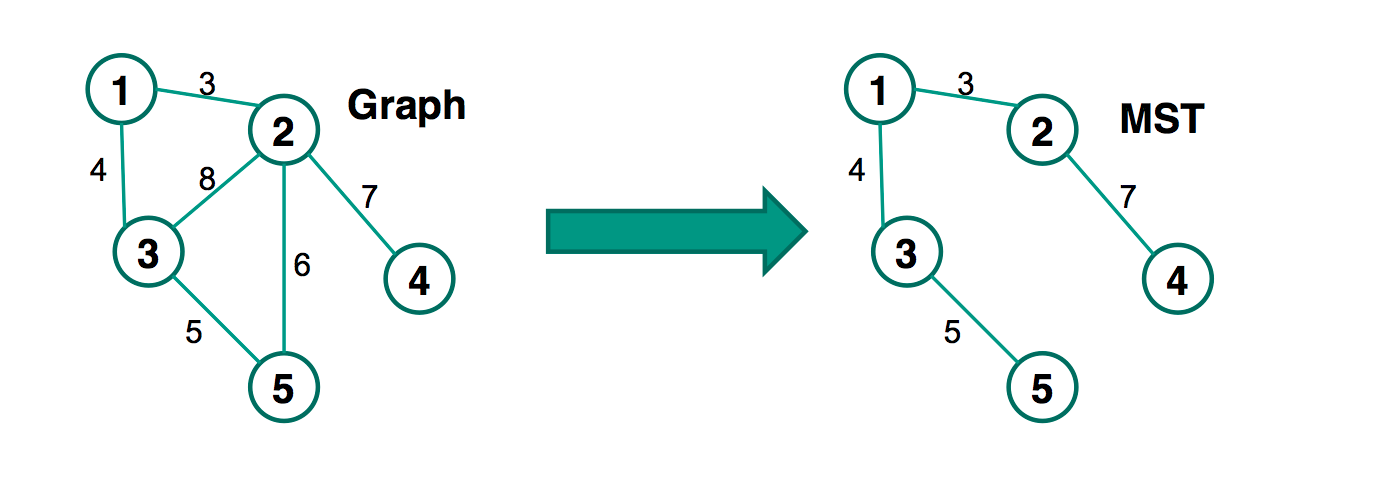
\includegraphics[scale = 0.25]{images/graphs}
\end{frame}

\begin{frame}{Schnitteigenschaft (Cut Property)}
	\begin{itemize}
		\item Für eine beliebige Knotenmenge $S \subseteq V$ sei $C$ die Schnittkantenmenge:
		$$C := \{ \{u,v\} \in E: u \in S, v \in V \  \textbackslash \  S \}$$

		\item Die Kante mit dem geringsten Gewicht aus $C$ ist im MST enthalten.
		\item Intuitiv klar, Teilmengen müssen irgendwo verbunden sein (formaler Beweis über Kreis in alternativem MST)
	\end{itemize}
\end{frame}

\begin{frame}{Kreiseigenschaft (Cycle Property)}
	\begin{itemize}
		\item In einem Kreis in dem Graphen ist die schwerste Kante nicht im MST enthalten.
		\item Auch intuitiv klar, man kann die Kante einfach weglassen
	\end{itemize}
\end{frame}

\begin{frame}{Aufgabe}
	Gegeben sei ein Graph $G = (V, E)$ mit Kantengewichten $\in \mathbb{N}$, die paarweise verschieden sind.

	\textbf{Aufgabe}: Zeige, dass der MST eindeutig bestimmt ist.
\end{frame}

\begin{frame}{Jarnik-Prim Algorithmus}
	\begin{itemize}
		\item Beginne MST beginnend bei einem Startknoten schrittweise auf
		\item Nutze die Schnitteigenschaft: Wähle immer die minimale Kante zwischen dem (wachsenden) MST und dem Restgraph
		\item Speichere zu jedem Knoten die Entfernung zum MST (Knoten im MST haben Entfernung 0)
		\item Zusätzlich verwalte Knoten in Priority-Queue, mit dem Gewicht der leichtesten Kante zwischen dem MST und dem Knoten
		\item Fast wie Dijkstra, also Laufzeit $\mathcal{O}((m + n) \log{n}$ bzw. $\mathcal{O}(m + n \log{n})$ mit Fib. Heaps
	\end{itemize}
\end{frame}

\begin{frame}{Jarnik-Prim Algorithmus}
	\begin{enumerate}
		\item Füge Startknoten in Priority-Queue $Q$ ein
		\item Solange $Q$ Elemente enthält:
			\begin{enumerate}
				\item Nimm minimalen Knoten $u$ aus $Q$ und füge ihn in den MST ein.
				\item Betrachte alle Kanten $(u, v)$ des Knotens.
				\item Für "`bessere"' Kanten füge $v$ in $Q$ ein oder aktualisiere die Priorität (Kantengewicht).
			\end{enumerate}
	\end{enumerate}
\end{frame}

\begin{frame}{Kruskals Algorithmus}
	\begin{enumerate}
		\item Sortiere die Kanten aufsteigend nach Gewicht
		\item Für jede Kante
			\begin{enumerate}
				\item Überprüfe, ob die Kante zwei Knoten verbindet, die schon im MST liegen
				\item Wenn nicht, füge die Kante zum MST hinzu
			\end{enumerate}
	\end{enumerate}
\end{frame}

\begin{frame}{Kruskals Algorithmus}
	\begin{itemize}
		\item Benutzt sowohl Kreis- als auch Schnitteigenschaft
		\item Entscheidend: Verwaltung der Teilmengen mit geeigneter Datenstruktur
		\item $\Rightarrow$ \textbf{Union-Find}
		\item Laufzeit: $\mathcal{O}(m \log{m})$ (beschränkt durch Sortieren)
	\end{itemize}
\end{frame}

\begin{frame}{Kreativaufgabe: Buy or Build}
	Gegeben ist eine Menge von Städten, die alle durch ein Netzwerk verbunden werden sollen.
	Zu jeder Stadt sind die Koordinaten gegeben, die Kosten um zwei Städte zu verbinden entsprechen dem Abstand.
	Zusätzlich existiert aber schon eine kleine Menge ($\leq 8$) von bereits vorhandenen Netzwerken, die gekauft werden können.

	\textbf{Aufgabe}: Wie kann möglichst effizient berechnet werden, wie hoch die Kosten sind um alle Städte zu verbinden? (Zunächst: wie kann die Aufgabe durch Graphen dargestellt werden?)
\end{frame}

\end{document}
